\chapter{Dialogic Human-AI Co-Creativity} \label{c:tc4}

This chapter addresses my core research question ("How can we design generative AI systems that act as effective co-creators, maintaining human agency while effectively leveraging the creative potential of this technology?") with a specific focus on research subquestion 2:
\begin{quote}
What is the potential of modeling dialogue in interaction design to enable effective human–AI co-creativity?
\end{quote}
It is presented in two parts.

The first part consists of a paper presented at the GenAI and HCI workshop at the 2022 Conference on Human Factors in Computing Systems (CHI 2022), which served as an initial exploration of how dialogue could enhance collaboration with generative AI, specifically Large Language Models (LLMs). At the time of writing, the dominant interaction modality with LLMs was text completion, where a model would complete a user-provided string of text. An emerging approach involved repurposing this function for linear instruction-following. In this paper, I explored taking the interaction a step further to engage with the model in a dialogic way. I argued that effective human-AI co-creativity requires the formation of mutual understanding of goals and intentions, and that dialogue can serve as the mechanism for this.

Through prompt engineering, I repurposed the text-completion function so that the model could interact in a bidirectional conversational exchange, enabling it to engage more as a co-creator rather than simply as a text-completion tool. A crucial aspect of this exploration was investigating the AI's ability to fluidly switch between meta-level dialogue about the creation (e.g., exchanging ideas, aligning goals) and object-level actions within the creation (e.g., writing, editing) in a single conversational thread.

A key output of this work was a typology of actions that both humans and AI could engage in during creative dialogue. These included generating new text, transforming or refining existing text, providing feedback, requesting clarification, and justifying decisions, among others.
This experiment was conducted in a freeform text interface and involved using an interface designed for text completion as a space for bidirectional dialogue. I argued that GUI elements were needed to scaffold such interaction.

This research preceded the widespread adoption of conversational interfaces; ChatGPT was launched six months after the presentation of this paper, leading to the rapid spread of bidirectional conversational interfaces as the primary form of interaction with LLMs. On one hand, this provided real-world evidence for the value of dialogic interaction. On the other hand, it also demonstrated that effective co-creativity requires more than simply a conversational interface.

The second part of the chapter explores what this entails. It presents a more recent and general framework for dialogue as an interaction design concept in co-creativity. Drawing on interdisciplinary scholarship, this section proposes that dialogic interaction comprises the following components:

\begin{itemize}
\item \textbf{Bidirectional Communication:} Two-way conversational exchanges.
\item \textbf{A Shared Space:} A common collaborative environment.
\item \textbf{Iteration:} The creative product and shared meanings evolve iteratively.
\item \textbf{Mutual Influence:} Each party’s perspectives and goals evolve as a result of the interaction, and each agent drives the other to new, unexpected directions.
\item \textbf{Mutual Understanding:} Each agent actively seeks to understand the other's world-models, goals, perspectives, and preferences.
\item \textbf{Context-awareness:} Actors bring in relevant context and act within it.
\end{itemize}

These components form an analytical lens for the subsequent chapters, which explore their implementation and their contribution to effective human-AI co-creativity.



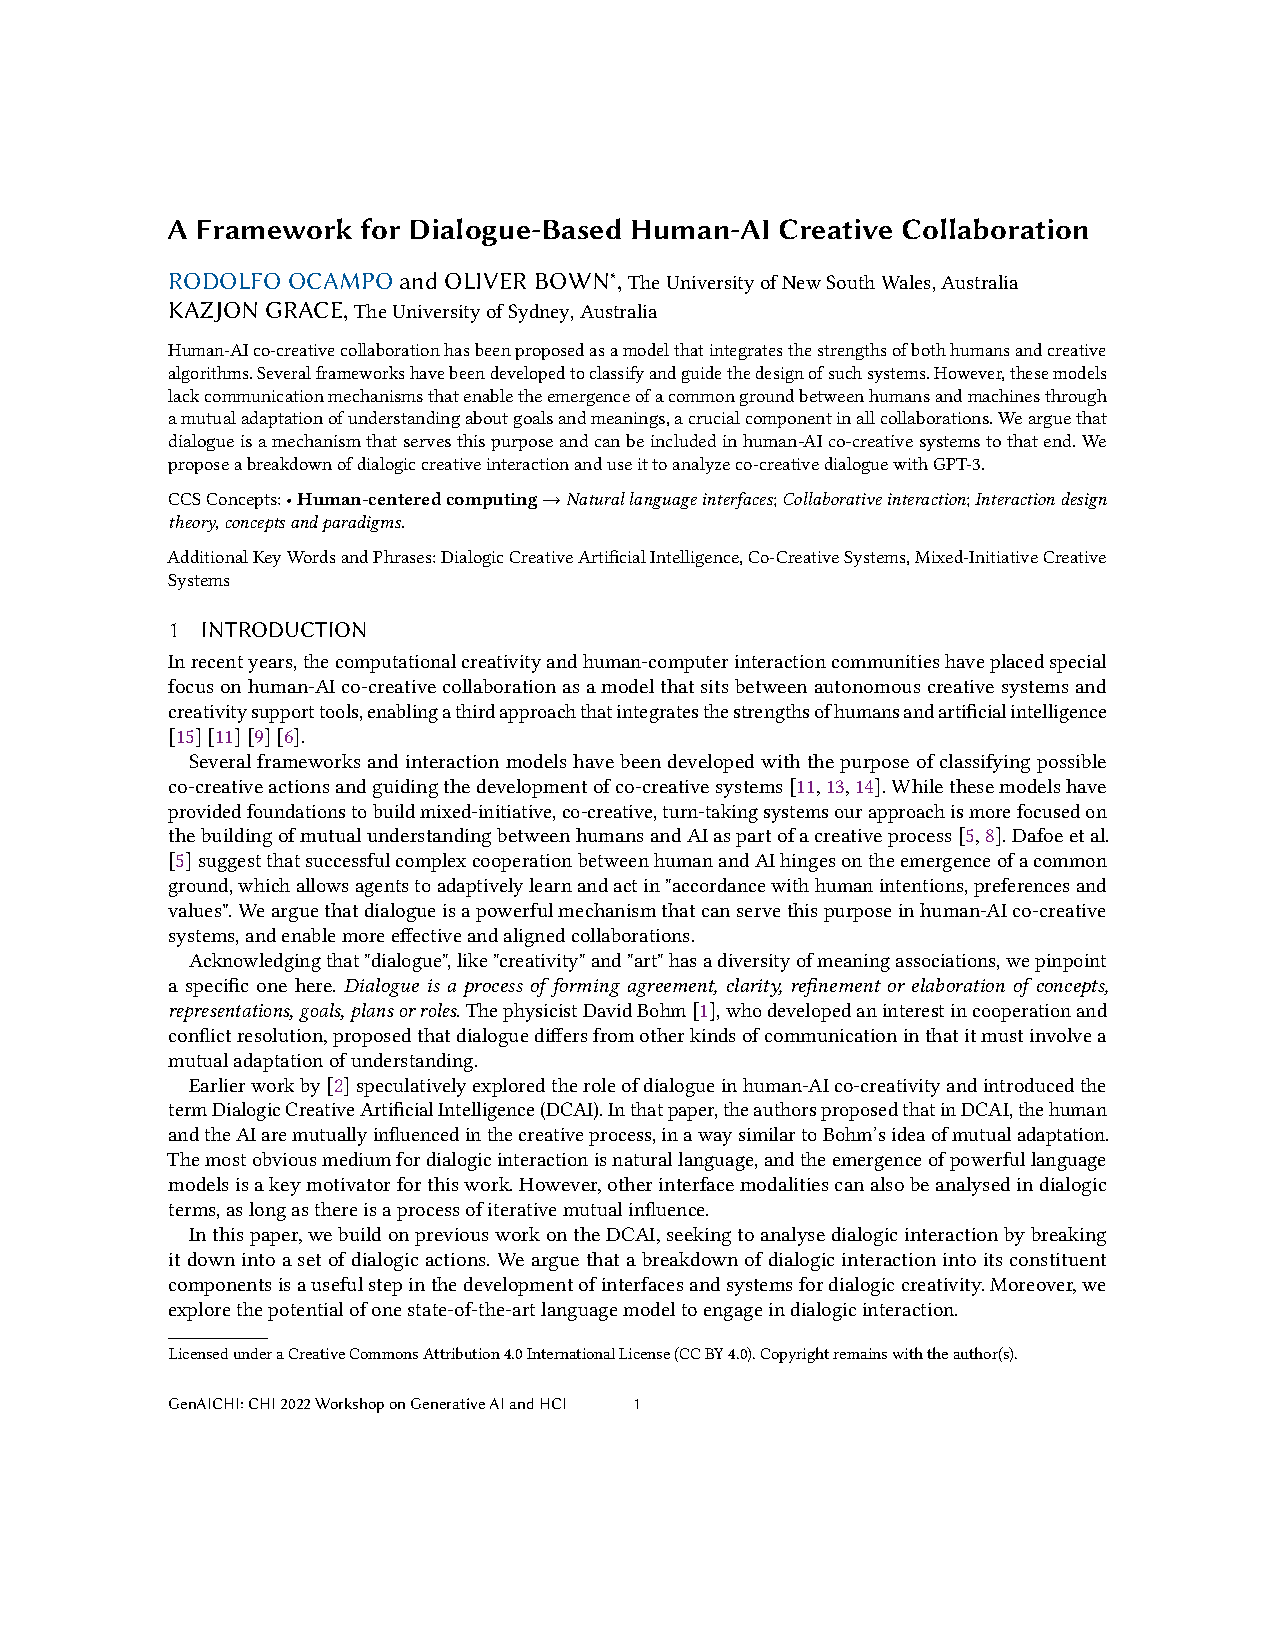
\includepdf[pages=-]{4-techchapter/GenCHI-thesis.pdf}

\section{Defining Dialogic Interaction as Human-Computer Interaction Concept}

Dialogue has been widely discussed in the context of human-computer interaction, mixed-initiative systems and co-creative systems \cite{Allen1999-sr, Yannakakis2014-zs, Deterding2017-wh} as a means to model human-computer interaction, however, it is yet to be formalised as both a theoretical concept and an actionable concept for interaction design. This chapter builds upon that work and on previous work by \cite{Bown2020-oc, Bown2024-yx}. As a unique contribution, in this chapter I seek to distill the elements that comprise dialogic interaction and how each can contribute to more effective human-AI co-creativity, thus providing a theoretical foundation for dialogic co-creativity as an interaction design concept. 

Dialogic interactions are based upon communication, iteration, feedback, adaptability, and deeper engagement, while non-dialogic interactions involve simple instruction giving or one-way communication, the sort one might observe commonly in computer-use paradigms such as command-based execution of tasks. For instance, in a dialogic interaction a writer might brainstorm with a language model, draft a story, request feedback on the flow, and iteratively refine the narrative—co-creating a text that neither agent could have produced alone. In contrast, in a non-dialogic interaction, the user may prompt the model in a command-driven way, to write a whole story. In this case, the involvement of the user is limited, which research shows may lead to worse quality, skill loss, and reduced task enjoyment \cite{Abbas2024-sf, Heersmink2024-mk, DellAcqua2023-og}. 

How to enable such dialogic interactions? At first glance, the question may seem trivially answered by chat-based interfaces. However, as I will discuss below, while chat-based interfaces certainly enable aspects of dialogic co-creativity, there are other important elements of dialogue that are not supported by such interface paradigms.

\subsection{Dialogic Co-creativity}

In 2020, \cite{Bown2020-zn} presented a speculative exploration of dialogue in human-computer co-creation, defining it simply as an interaction in which both actors influence each other. More recently, in \cite{Bown2024-yx}, we introduced a more comprehensive and formal framework for dialogic interaction, distinguishing among three levels: pseudo-dialogue, weak asymmetric dialogue, and full dialogue.

In \textbf{pseudo-dialogue}, the human provides instructions to the computer, which then generates an output for the human to evaluate. The interaction remains largely one-directional, as only the human models the AI; there is no cycle of mutual influence or shared intentions, and the channels for iterative, context-aware collaboration are limited. By contrast, \textbf{weak asymmetric dialogue} allows for some degree of bidirectional communication, but the computational agent’s capacity to model the interaction space is constrained. Although the communication may flow both ways, the relationship largely reflects a client-producer dynamic, with limited reciprocal understanding.

Finally, in \textbf{full dialogue}, both the human and the computer actively model each other. They engage in bidirectional communication that is aware not only of the immediate conversation but also of the broader collaborative context. This iterative process continuously refines the creative output while also deepening the mutual understanding between human and AI. 

In the following sections, I examine the elements that characterise \textbf{full dialogue}. The absence of one or more of these elements corresponds to instances of pseudo-dialogue or weak asymmetric dialogue.

\begin{figure}
    \centering
    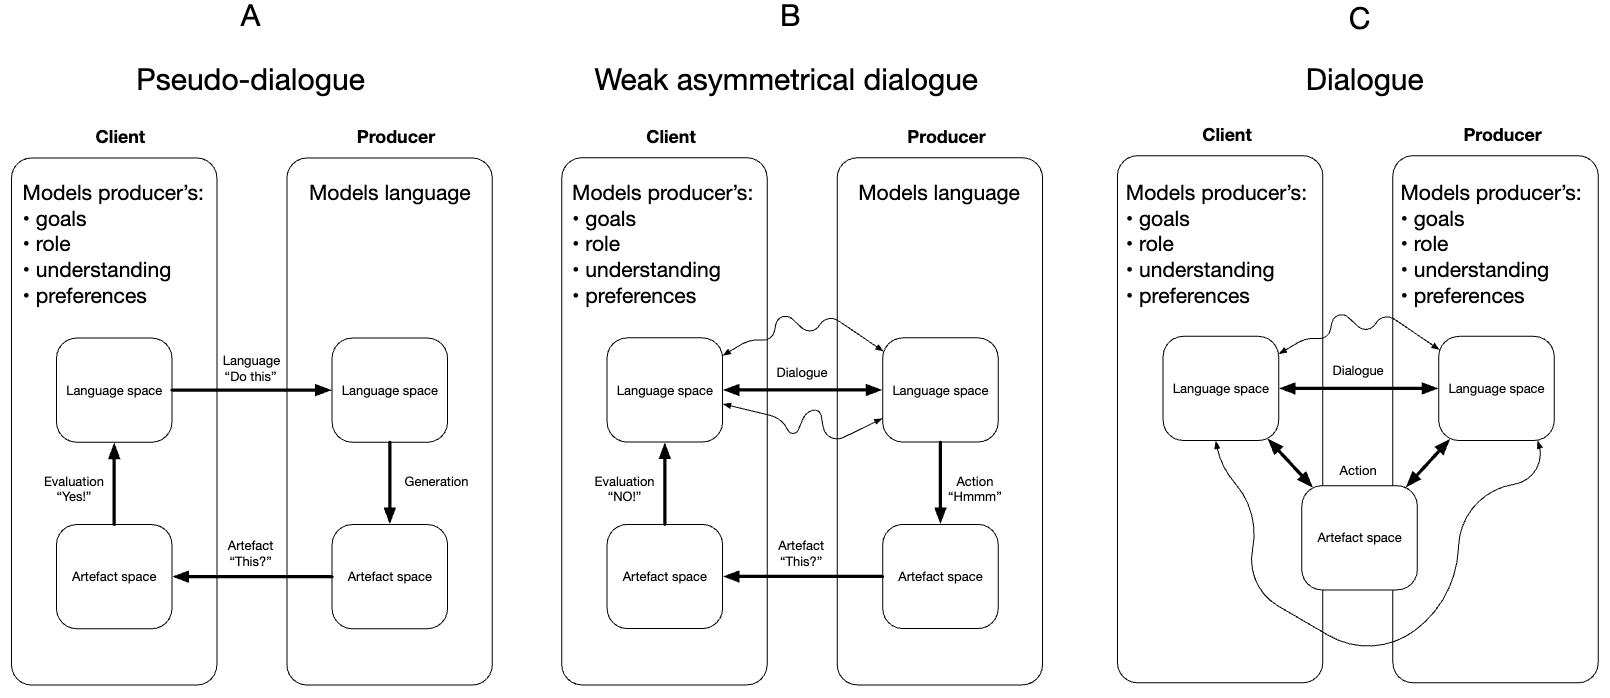
\includegraphics[width=1\linewidth]{levels of dialogue.png}
    \caption{Three levels of dialogic interaction. In weak-asymmetric dialogue, only the user models the AI who produces outputs based on prompts or requests. In pseudo-dialogue, a level of communication takes place but the collaboration and mutual modelling is limited. In full-dialogue, both model each other and act and evaluate the common creation.  Figure from \cite{Bown2024-yx}}
    \label{fig:enter-label}
\end{figure}
\subsection{Elements of dialogic co-creativity}

Drawing from the broader literature in philosophy, education, and HCI, I distil the following key elements of dialogic co-creative interaction. 

    \begin{itemize}
        \item Interaction \textit{through} and \textit{about} the creation, which involves: 
        \begin{itemize}
            \item Bidirectional Communication: Two-way communicative or conversational exchanges.
            \item A Shared Space: There is a common collaborative environment separate from instructions or chat interfaces.
        \end{itemize}
        \item Mutual Influence: Each party’s perspectives and goals evolve as a result of the interaction and each agent drives the other to new unexpected directions.
        \item Mutual Understanding: Each agent actively seeks to understand the other's world-models, goals, perspectives, preferences, etc.
        \item Iteration: The creative product and the shared meanings evolve iteratively.
        \item Context-awareness: Actors bring in the relevant context and act within it.
    \end{itemize}


    \begin{figure}
    \centering
    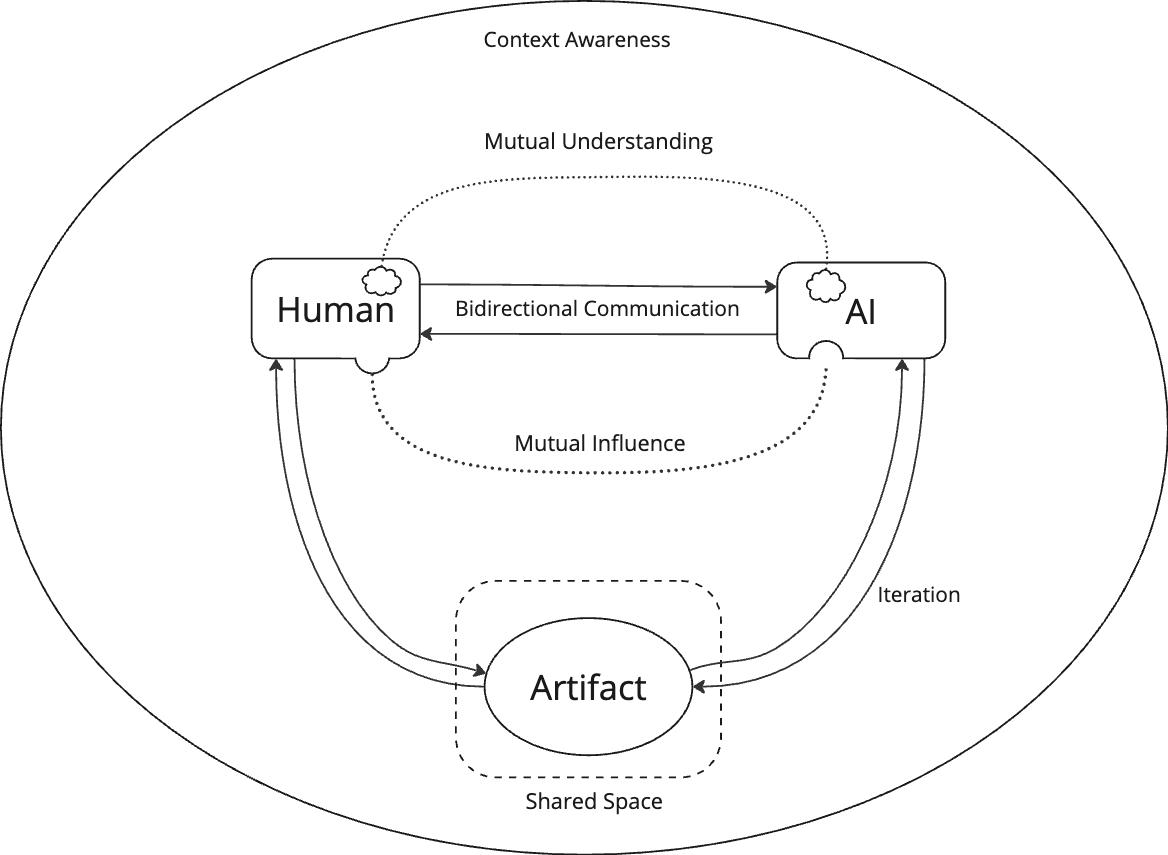
\includegraphics[width=0.75\linewidth]{dialogicelements.png}
    \caption{Dialogic co-creativity as an interaction design concept is comprised of six
essential elements: bidirectional communication, iteration, mutual influence, mutual understanding, shared space and context-awareness. }
    \label{fig:enter-label}
\end{figure}


In the next section, I elaborate on each element and discuss how each principle can improve human–AI co-creative outcomes, drawing on empirical evidence. By examining real-world examples and research findings, I highlight how dialogic features address frequent shortcomings of generative AI interactions—such as lack of nuanced steering, iterative dynamics and reduced user engagement.

\subsubsection{Bidirectional Communication}

One defining characteristic of dialogue is \textit{bidirectional communication}. Although such communication typically occurs through natural language, dialogue need not be constrained by verbal interaction alone. Etymologically, “dialogue” derives from the Greek words \textit{dia} (through) and \textit{logos} (word), yet several theorists maintain that dialogue can extend beyond mere language. For instance, the dialogic philosopher \cite{Buber1923-us} posits the possibility of dialogue occurring between humans and non-humans, while Donald Schön describes design as a dialogue among the creator, the materials, and the environment, in which iterative cycles of action and reflection incrementally shape the outcome \cite{Schon1987-fy,Schon1992-jt}. Within such a framework, dialogue functions as a cycle of mutual influence wherein information flows \textit{both} ways.

Other scholars, however, emphasize the importance of natural language for successful interaction between humans and sophisticated computational systems. Hayes and Reddy, in the early days of computing, advocated that "gracefully interacting systems" need to “conduct a dialogue in as human-like a way as possible,” highlighting the need to resolve linguistic ambiguity effectively \cite{Hayes1983-ca}. Much of their empirical work examined simpler systems lacking today’s advanced dialogic capabilities, but their core argument remains prescient: clear communication is critical for interacting with and understanding advanced systems.

\textbf{Empirical Evidence Supporting Bidirectional Communication}

Empirical support for the value of bidirectional communication in human–machine co-creation emerges from several studies. First, \cite{Rezwana2022-gg} compared two co-creative systems: one featuring bidirectional human–AI communication and another restricted to one-way (human-to-AI) interaction. Their findings showed that the bidirectional design improved user engagement, perceptions of the AI’s intelligence, and a more positive collaborative experience. Users reported that the AI felt more like a \textit{partner} than a mere tool, citing its ability to offer feedback and tailor outputs to user preferences. 

A second study, \cite{Ashktorab2021-ie}, investigated communication directionality in a cooperative game setting. The researchers found that systems capable of dynamically responding to user inputs—thus engaging in bidirectional communication—were viewed as more intelligent, likable, and conducive to rapport. By adaptively adjusting responses based on user prompts, the AI demonstrated a kind of non-verbal, iterative feedback loop. Conversely, systems with one-way communication were perceived as less cooperative and gave users a diminished sense of control.

A final, real-world illustration of two-way dialogic interaction is ChatGPT. The service, which became the fastest-growing consumer application—reaching 100 million registered users within two months and 300 million active users by December 2024—highlights the profound user appeal of conversational design. Notably, the underlying technology (GPT-3.5) had been available earlier, but as OpenAI President Greg Brockman explained in an interview when asked why ChatGPT became so successful, he claimed that ChatGPT’s interface was intentionally redesigned for \textit{dialogic} exchange. "we actually had the technology behind it (GPT3.5) the model behind it created almost a year prior so it wasn't new technology, the thing that we really did differently is that we did a little bit of extra work to make it more aligned so it really you could talk to it and it would do what you wanted, but secondly we made it accessible. We built an interface that was super simple. It was kind of the simplest interface we could think of." Brockman claims that the biggest take away is through this changes, they were able to "see the gap between what people thought was possible and what actually had been possible for quite some time" \cite{SXSW2023-wg}.Rather than merely offering text completions, ChatGPT was trained and fine-tuned (via Reinforcement Learning from Human Feedback, RLHF) to sustain a \textit{conversation}. 

\textbf{From Text Completion to Dialogic Interaction}

The evolution of GPT-based systems reveals a progression in dialogic interactivity. Early language models such as GPT-2 and GPT-3 operated in a predominantly \textit{text-completion} mode, offering no clear bidirectional exchange \cite{Brown2020-js}. Subsequently, \textit{instruction-based} models—exemplified by InstructGPT—enabled \textit{human-to-AI} communication by parsing user instructions \cite{OpenAI2022-pj}. Finally, with the introduction of ChatGPT, \textit{AI-to-human} communication also became formalised: the system now produces conversation-like “responses,” effectively completing a loop of bidirectional dialogue \cite{OpenAI2022-wx}.

\begin{table}[h!]
\centering
\resizebox{\textwidth}{!}{%
\begin{tabular}{|l|p{7cm}|l|}
\hline
\textbf{Interaction Model}         & \textbf{Description}                                                                                          & \textbf{Level of Communication}   \\ \hline
Text-Completion (e.g., GPT-3)      & No communication: The model completes text based on a provided input string. No back-and-forth communication. & None                             \\ \hline
Instruction-Based (e.g., InstructGPT) & One-way communication: The user provides an instruction, and the model completes it. Interaction is directive but linear. & Human-to-AI                      \\ \hline
Dialogic/Chat-Based (e.g., ChatGPT) & Two-way communication: The AI engages in conversational dialogue, responding to user inputs as part of an iterative conversation. & Human-to-AI and AI-to-Human       \\ \hline
\end{tabular}%
}
\caption{Progression of Communication Models in Generative AI}
\label{tab:communication_progression}
\end{table}

While chat-based, conversational, and dialogic language models have greatly increased the usability and adoption of AI-driven language technologies, they remain limited in their ability to serve as true co-creators. Among these challenges are the difficulty of detecting subtle nuances and fully grasping users’ intentions \cite{Bown2024-yx}, the propensity of models to fabricate information (“hallucinate”) \cite{Alkaissi2023-tp}, and the lack of dedicated spaces for co-creative processes beyond the chat interface \cite{Ocampo2024-dv}. In addition, these systems are not always sufficiently critical, often complying with user instructions despite erroneous underlying assumptions. I will return to these limitations in subsequent sections.


\begin{figure}
    \centering
    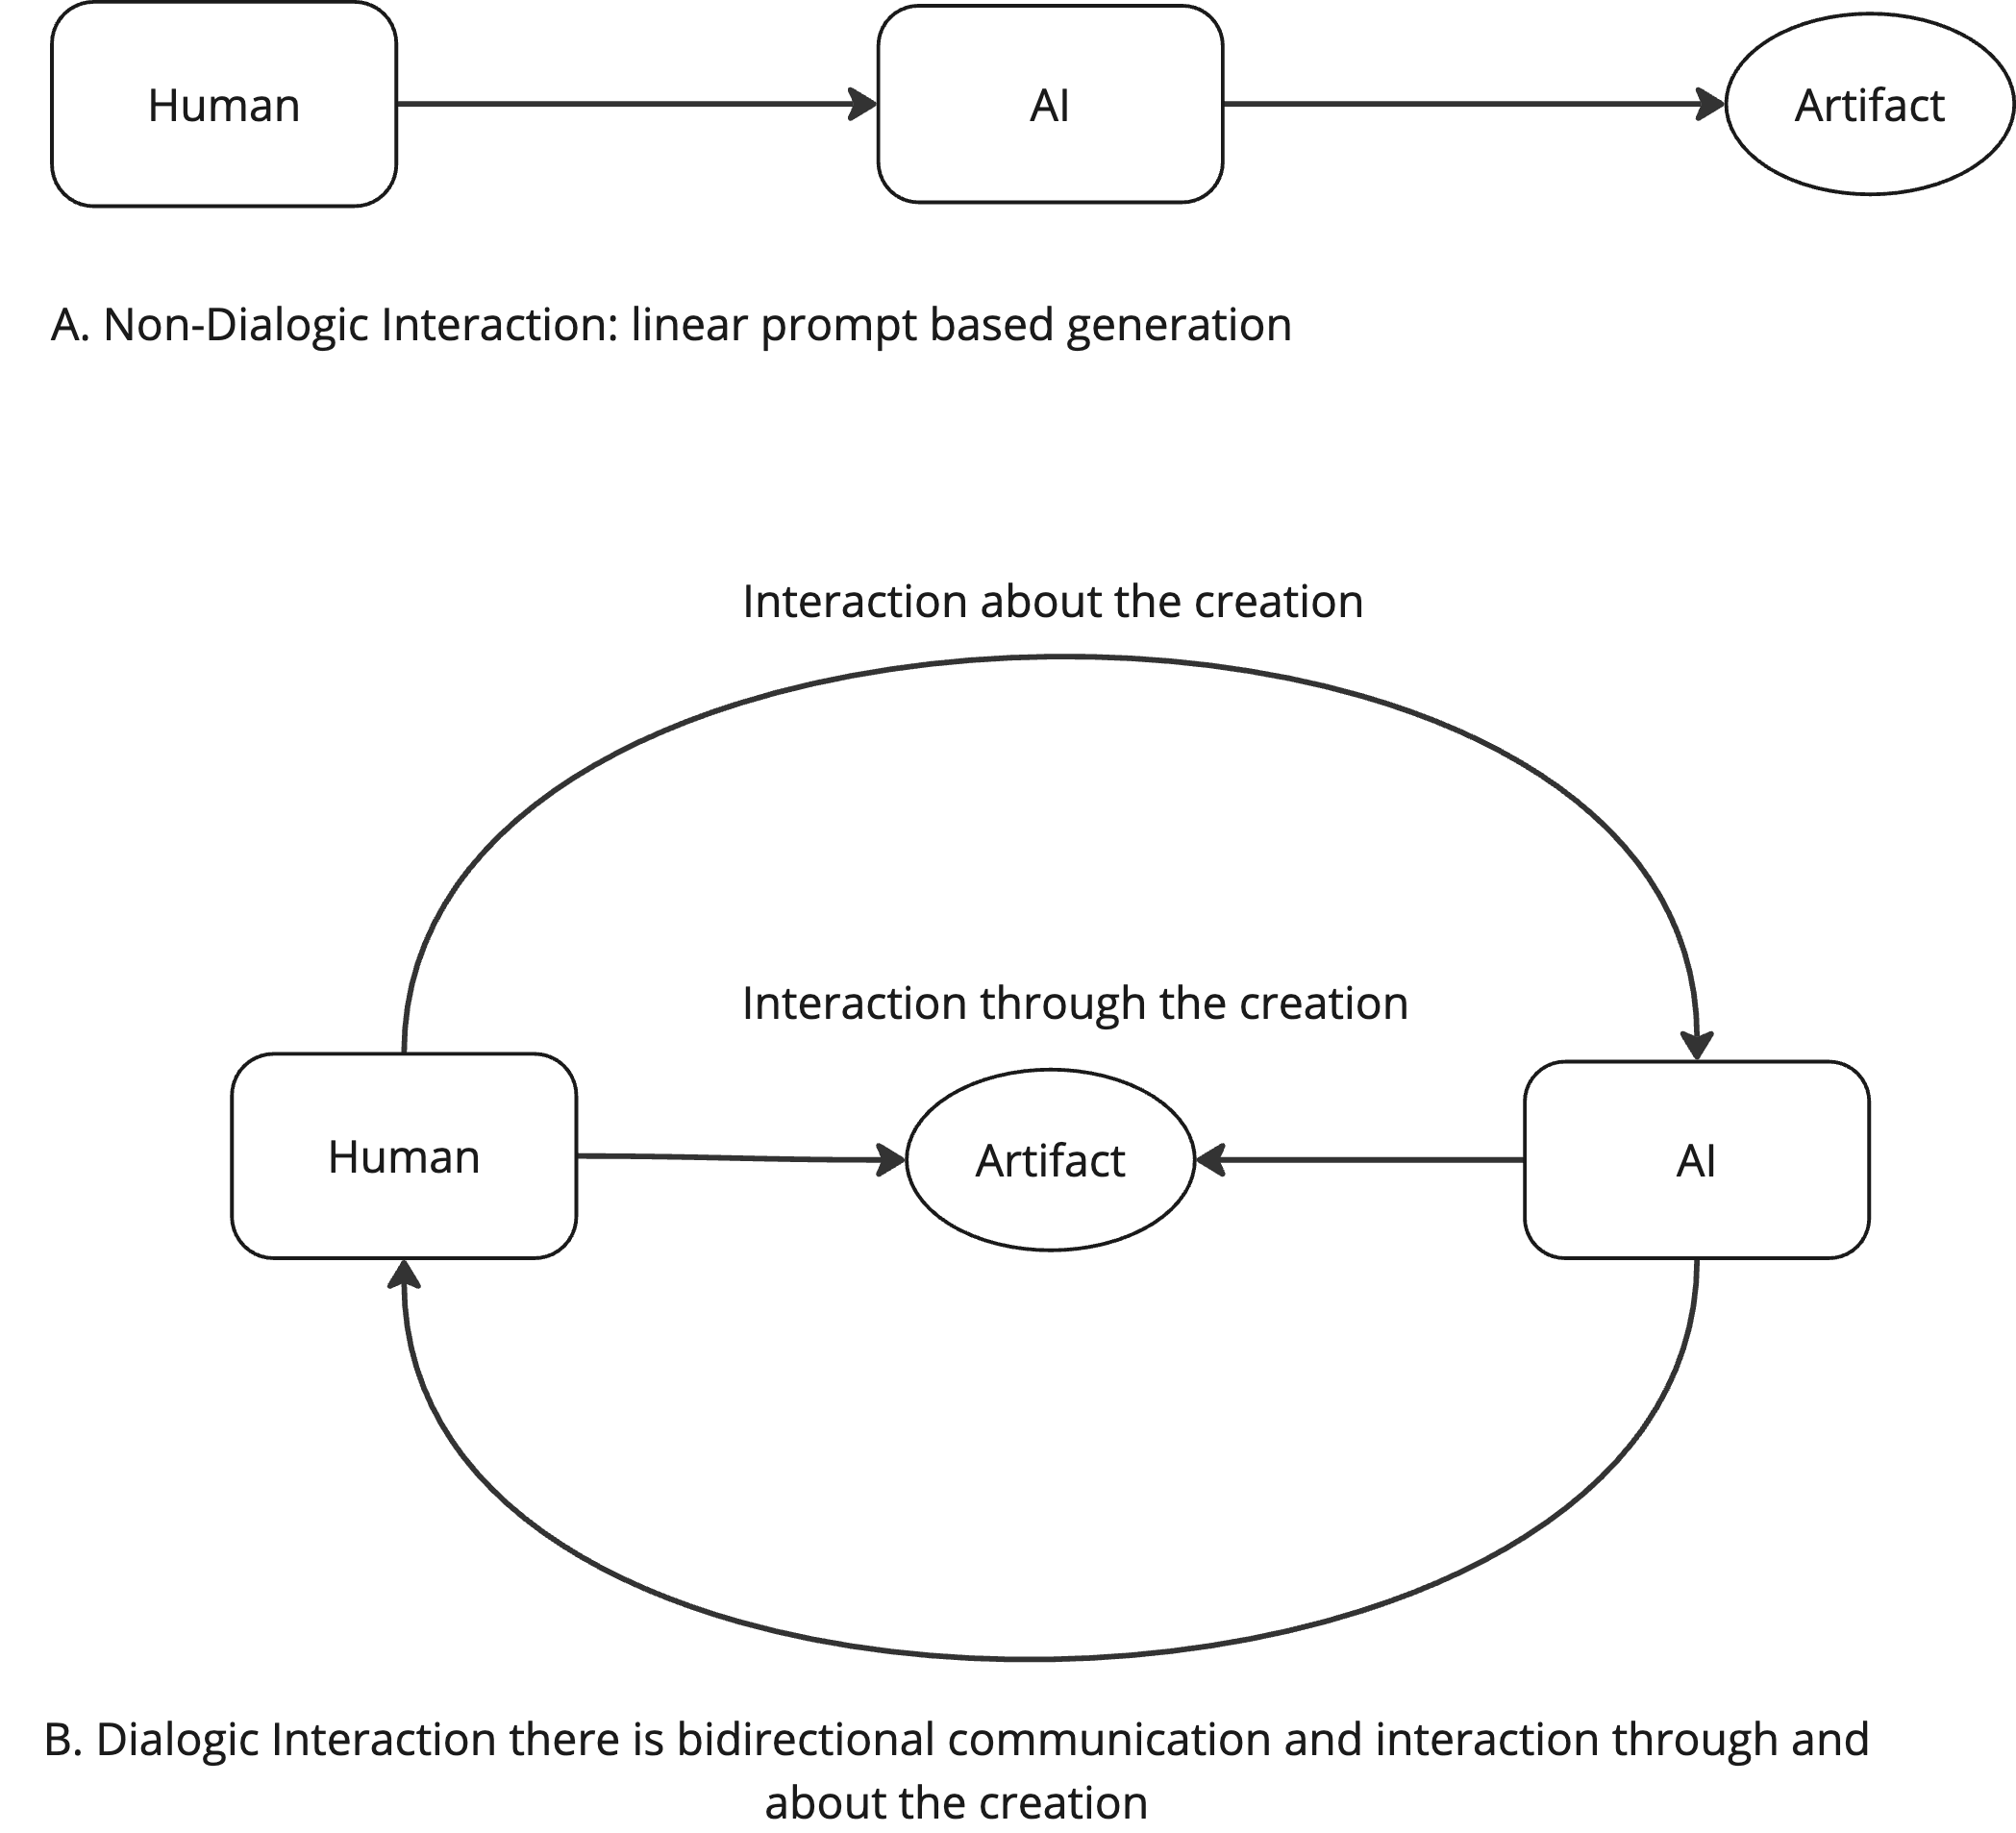
\includegraphics[width=0.75\linewidth]{Bidirectional.png}
    \caption{Interactions that enable two-way communication are important for effective co-creative dialogic interaction}
    \label{fig:enter-label}
\end{figure}

\subsection{Mutual influence}

Bidirectional communication is foundational for dialogic interaction, yet natural language exchanges alone do not guarantee effective co-creation. A key element is \textit{mutual influence}—the capacity for both parties to shape each other’s perspectives, goals, or actions \cite{Bown2020-zn}. In genuinely creative dialogue, participants provoke each other to reconsider their stances thus creating something \textit{new} that neither had created before the interaction. By contrast, non-dialogic exchanges exhibit limited mutual influence and primarily involve one-directional persuasion, as in giving orders, instructions, or arguing with the sole intention to convince.

A salient example of mutual influence in dialogue—and its importance for successful co-creation—appears in the Socratic dialogic method, one of the foundational applications of dialogue as an interaction technique. Unlike classical philosophical approaches such as sophist rhetoric or debates, whose aim was to persuade others of a particular viewpoint, the Socratic dialogic method functioned as a collaborative process of shared discovery. Socrates called his approach an “intellectual midwifery” designed to “give birth to a person’s inner wisdom” through critical thinking and the co-production of knowledge (although some dialogues ended in \textit{aporia}, or impasse) \cite{Nails2005-iq, Wikipedia-contributors2024-hr}. Participants typically began by posing a fundamental question, then iteratively questioned one another, proposed alternative viewpoints, refuted logically unsound positions, and ultimately arrived at a conclusion. The Socratic method was creative at two levels: first, it often, but now always, arrived at new philosophical solutions. More importantly, however, its aim was to modify the entrenched perspectives of interlocutors. Modelling this process is useful for enabling emergent creativity in human-AI interactions.

While some generative AI models demonstrate strong conversational abilities, they often fail to engage in questioning or actively seek to induce perspective shifts—except, for instance, when handling malicious queries. This behaviour is largely a result of alignment training for safety, in which models are optimised to comply with user instructions. However, in human-human co-creative dialogue, such reciprocal questioning and openness to influence are crucial.

A case study by \cite{Bown2020-oc} offers a practical illustration of how mutual influence shapes a creative process. In this study, two musicians co-created a song by offering alternative perspectives to each other. For instance, one musician (A) took a break and listened from outside the room. After hearing something interesting, he returned, declaring “That’s the hook!” Musician B, surprised, pointed to a different section and responded, “Oh, really, I thought \textit{that} was the hook.” B insisted, “No, no, \textit{that’s} the hook.” This exchange reveals how co-creators profit from actively exchanging viewpoints, prompting each participant to question their own assumptions. Tools like Oblique Strategies leverage a similar principle: they deliberately provoke shifts in perspective, offering oblique, unexpected suggestions that challenge the current framing. From the perspective of the psychology of creativity, this is particularly relevant, since one of the main obstacles in creative processes is hyperfixation in a particular solution or framing that leads to creative blocks \cite{Jansson1991-wy}. 

By contrast, most generative AI systems do not support this dynamic of mutual influence. More often, they conform to user instructions, potentially leading to less creative outcomes. Research has shown, for example, that ina  case study of image and design generation, using generative AI systems as part of a creative process led to greater fixation and less creative results than not using the system \cite{Wadinambiarachchi2024-jn}. 

Striking a balance between AI systems that actively question users and those that remain safe, aligned, and responsive is challenging. One promising direction may be to design systems that actively seek to introduce perspective shifts, and question the user productively, while allowing users to adjust parameters that govern this behavior. 

For example, consider a scenario in which a dialogic, multimodal co-creative musical AI system collaborates with a user composing commercial music. If the user plays a chord progression ending on a D\# in the key of E major and says, “Help me continue from here,” the system could move beyond simply following the prompt. It might propose a more adventurous move, for example: “What if, instead of finishing on D\#, you transition to an F\#7 to create additional tension? From there, we could resolve to a B major for an unexpected yet refreshing resolution.” This recommendation not only complies with the user’s request but also encourages rethinking—enriching the co-creative output.

Increasingly, interactive systems that incorporate some of these principles are appearing in both the literature and practice. For example, \cite{Kim2023-wt} describes the Scraft co-creative writing tool, which uses a language model as a “thought-provoking” tutor. It employs a Socratic questioning style to guide students toward deeper thinking and improved writing skills. Similarly, in “Do Make Me Think!” \cite{Reicherts2020-up} demonstrates how conversational interfaces that challenge users can scaffold cognitive processes, enabling them to discover new perspectives or previously overlooked trends. In 2019, \cite{Karimi2019-io} introduced a co-creative system for drawing that actively seeks to introduce novelty and perspective shifts by intentionally varying the visual and conceptual similarity with increasingly more novelty 

Mutual influence depends greatly on each party’s willingness to be influenced rather than simply to influence the other \cite{Bohm1996-fo}. Systems that question users to stimulate critical thinking and promote reciprocal engagement may help offset the risks of skill and critical-thinking erosion associated with overly compliant generative tools \cite{Abbas2024-sf, Essel2024-qc}. Nevertheless, the task is to achieve an appropriate balance between challenging users and following their instructions.

On the other hand of mutual influence is the influence flowing from the human to the AI. In what ways does the human influence the AI? In a seemingly trivial case, they exert influence merely by inputting prompts and requests thus producing an output by the AI. However, this seemingly trivial case actually disguises the more complex problem of control and steerability in generative systems, which I cover in more detail in subsequent chapters.

\subsection{Mutual Understanding}

A further essential facet of dialogic interaction is \textit{mutual understanding}, which Bohm describes as the process of modeling each other’s perspectives \cite{Bohm1996-fo}. Whereas mutual influence entails shaping each other’s views or actions, mutual understanding involves establishing a shared conceptual frame. Dialogue, in this sense, serves as a pathway to aligning and generating new, \textit{common} meanings. In his influential work on dialogue, Bohm posits that co-creativity emerges in the space where these new meanings form \cite{Bohm1996-fo}. Participants enter a dialogue with different worldviews—variations in how they define and interpret concepts—and these discrepancies can impede collaboration. Dialogue can rectify these misalignments, forging a common ground from which genuinely co-creative outcomes can arise.

Translating this principle to human–AI co-creativity highlights how both humans and AI bring distinct world-models into an interaction. Humans draw on lived experiences, while AI relies on patterns learned from vast training data, encoded within latent spaces. Inevitably, differences in how each interprets or values certain concepts can lead to misaligned objectives or aesthetics.

For instance, imagine a user prompting an AI to generate an image of a “beautiful house.” The system then produces a sleek, modern design, but the user—who prefers rustic, cozy homes—objects, remarking, “No, that’s ugly! Generate something made of wood, resembling a cabin.” In an ideal scenario, the model would learn that the user associates modern architecture with ugliness and rustic aesthetics with beauty. Yet many current generative models have limited capacity to internalise these user-specific preferences. In another example, \cite{Bown2024-yx} showed that model was unable to succesfully grasps the user preference for "witty" and sarcastic styles for crafting a tagline, significantly limiting its ability to successfully help the user. 

On the other hand, user's understanding how the system works is equally important. Research on \textit{explainable AI} suggests that systems capable of clarifying their reasoning or representations foster more effective interactions and user trust \cite{Ribeiro2016-xb,Doshi-Velez2017-qv}.

Significantly, mutual understanding need not be confined to verbal communication. Humans and AI can learn from each other iteratively through the creative process itself. In image generation, for example, the AI’s latent space determines how conceptual attributes (e.g., style, structure, or mood) are encoded. Co-creation may be viewed, then, as a form of \textit{latent-space exploration} \cite{Loh2024-fb,Smith2022-dm}, yet users often lack a concrete map of how to navigate these underlying representations. Some approaches attempt to render latent spaces semantically navigable, allowing users understand it and thus succesfully explore it \cite{Prathyush2024-ly, Harkonen2020-eu, Davis2024-ml}. By exposing the latent space in a more interpretable manner, these interfaces help users build more accurate mental models of the system.

Conversely, the system can learn (or at least simulate learning) about user tastes and implicit goals. For example, \href{app.leonardo.ai/}{Leonardo’s Flow State} prototype presents a grid of image variants; users pick one they like, then generate similar versions, effectively drilling deeper into the region of the latent space that aligns with their preferences. Such iterative sampling and selection not only refines outcomes but also promotes mutual understanding by enabling the AI to \textit{adapt} to the user’s evolving sense of aesthetic goals and constraints.

\subsection{Iteration}

Iteration is a key aspect of dialogic interaction, whereby participants take turns contributing and collaboratively refining ideas or outputs. Similarly, iteration underpins creative processes, as creators progressively refine their work through divergent and convergent stages. However, generative AI currently lacks robust mechanisms for iterative interaction, limiting its potential as an effective co-creative system. Indeed, a deficiency of iterative dynamics is frequently cited as a core constraint on generative AI’s co-creative utility, particularly in non-text-based tasks such as image creation \cite{Park2024-gw, Ocampo2023-gu, Peng2024-tr}. Consequently, designing iterative capabilities remains critical for advancing human–AI co-creativity.

The evolution of large language models (LLMs) illustrates the potential of iterative interaction. Over time, LLMs have progressed beyond non-communicative modes and one-way text completion toward dialogic, iterative modalities. These modes enable users to refine outputs by requesting modifications, expanding the AI’s suggestions, or clarifying goals. Nevertheless, significant limitations persist in these iterative processes \cite{Bown2024-yx, Ocampo2024-dv}.

At present, non-text-based generative systems lag behind LLMs in their ability to support iterative dynamics. This gap arises from both technical constraints and interaction-design challenges related to maintaining consistency, control, and refinement of outputs \cite{Ocampo2024-dv}. Consider, for example, a designer seeking to modify a newly generated sofa design. While the designer might like the core design, they may wish to make the sofa thinner or alter certain features. However, simply requesting such specific changes is rarely feasible: the designer can only attempt to re-prompt using the existing output as a reference, which may or may not yield a satisfactory result. Although emerging approaches—such as InstructPix2Pix \cite{Brooks2022-vo} and omnimodal foundational models \cite{Pichai2024-ao}—aim to address these issues, truly robust iterative refinement remains elusive.

From an interaction-design perspective, however, iterative dynamics are already achievable by structuring tools and workflows around multiple rounds of refinement \cite{Koch2020-gx, Lee2022-rj, Kim2023-wt}. For instance, systems can provide explicit feedback loops, where outputs become inputs in subsequent iterations.

Park et al. \cite{Park2024-gw} demonstrated that an exploratory GAN-based tool can better facilitate iterative image refinement than a single-step, text-to-image system like Stable Diffusion. Lee et al. \cite{Lee2022-rj} further showed that emphasising iterative interaction (rather than one-shot outputs) yields richer insights into users’ co-creative experiences. In a complex consulting task, Dell’Acqua et al. \cite{DellAcqua2023-og} found that consultants who engaged in tight, iterative feedback loops with an AI model outperformed those who interacted sporadically or relied on one-step solutions. Overall, the usability of generative AI depends heavily on its capacity to foster iterative dynamics, highlighting the importance of dialogic interaction in co-creative contexts.

\subsection{Shared Space}

Dialogic co-creation relies on a shared space in which participants can collaboratively contribute and refine artifacts. Paulo Freire, a central figure in dialogic education, emphasises the importance of dialogic space as a cornerstone of his pedagogical method \cite{Freire1970-pa}. How might this apply to human-AI co-creativity?

Consider the example of a writer collaborating with a chat-based language model, such as Claude or ChatGPT. The writer might begin with an initial draft and ask the AI to improve it. To further refine the text, the user must copy and paste the updated content back into a text editor, make any changes, and—if they wish to continue working with the model—reinsert the revised text into the chat. This repetitive process introduces significant friction, often discouraging the user from fully participating in iterative co-creation. Instead, they might accept the AI’s first suggestion and move on, leading to potential overreliance and a diminished sense of ownership. Evidence suggests that minimal user involvement can result in decreased performance, loss of personal style, skill erosion, and increased errors \cite{Abbas2024-sf, Rafner2021-tm}.

In two studies conducted across 2023 and 2024 during my doctoral research, I explored the impact of an interface I designed that offers both a chat window and a collaborative writing space shared by the user and AI. In this environment, both the user and the AI can read, write, and edit the text. Compared to conventional chat interfaces, this setup increased user involvement and strengthened their sense of ownership. It also shifted the collaboration dynamic away from a client-producer model, in which tasks are “outsourced” to the AI, and toward a more reciprocal co-creative relationship \cite{Ocampo2024-dv}.

Recently, chat-based AI tools have begun introducing features that support a shared space more seamlessly. For instance, Claude’s “artifacts” feature provides a dedicated area for text and code separate from the main chat window; however, the user cannot make changes in this space, only the AI can \cite{Whitney2024-pp, Anthropic2024-dl}. ChatGPT’s “Canvas” likewise creates a co-creative workspace where user and AI can jointly read, write, and edit text-based content \cite{OpenAI2024-ug}. These emerging designs represent early steps toward more robust shared spaces that foster deeper, more integrated human-AI co-creativity.

\subsubsection{Context Awareness}

A final crucial component of dialogue is what I refer to as context-awareness. Dialogic exchanges are interpreted not only in light of the immediate interaction but also through broader contextual factors. For example, Lucy Suchman \cite{Suchman2006-bs} illustrates how even a seemingly straightforward question—“Are you going to be here in ten minutes?”—and the response “Go ahead, take your break” rely on a larger contextual understanding implicitly known and not expressed in the current conversation. 

Similarly, creative practices are embedded within networks of meaning that extend beyond the present co-creation. Under an evolutionary lens of creativity, individuals respond to environments that are socially, culturally, and technologically constructed \cite{Bown2021-os}. Competencies to act within these environments include factors such as taste and trend awareness, alongside more practical artistic skills.

Consequently, a successful co-creative dialogue between humans and AI must be properly situated within the relevant context, which can happen at different levels. On one level, it may involve contextual awareness of past interactions, as well as the context awareness of the user workspace including previous works, files, context and preferences. On another wider level, it can involve a broader cultural context including awareness of current trends and social considerations that inevitably shape creative processes and the value of artifacts.

Consider for example, a designer using a co-creative image generation system to ideate designs for a fashion collection. Ideally, the designer would be able to reference their own style and past collections, as well as generating designs that are aware of the seasonal trends. Currently, the capacity for image generation systems to enable this is limited.

Consider a second example: a programmer collaborating with an AI language model to write code. In this case, ideally, the AI is integrated into the coding environment so that it can be aware of the existing codebase, dependencies, and the ability to create new files. 

\begin{figure}
    \centering
    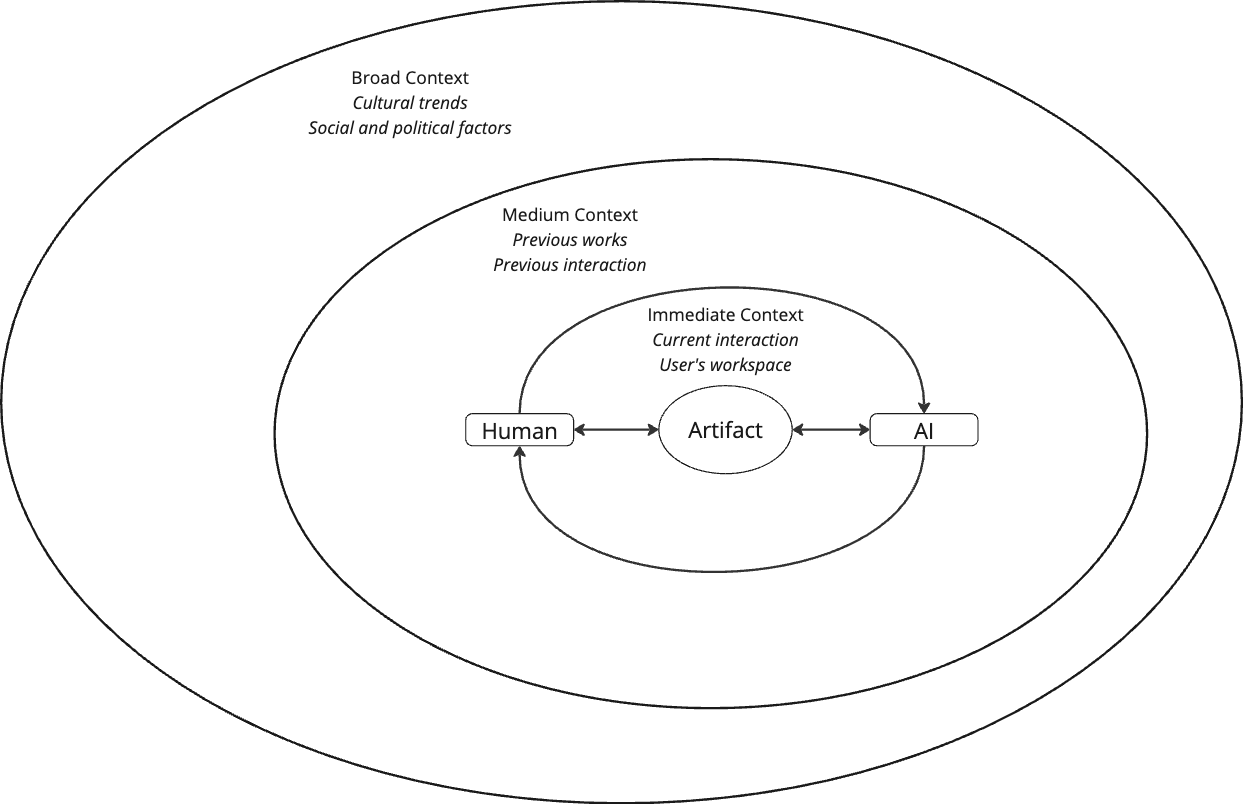
\includegraphics[width=0.75\linewidth]{context.png}
    \caption{Effective co-creative dialogues consider context at different levels}
    \label{fig:enter-label}
\end{figure}

Several emerging AI tools are advancing toward context-awareness and integration to varying degrees. \href{https://www.cursor.com/}{Cursor}, \href{https://v0.dev/}{v0}, \href{https://replit.com/ai}{Replit’s AI agent}, and \href{https://github.com/features/copilot}{GitHub Copilot} integrate directly into coding environments, enabling them to reference relevant files, generate new code, create additional files, and even handle deployments. \href{https://www.canva.com/}{Canva’s DreamLab} and \href{https://www.adobe.com/au/products/firefly.html}{Adobe} introduce generative AI within design workspaces, facilitating context-aware functionality. Google’s Gemini Workspace similarly seeks to integrate its features into users’ workflows across email, documents, and other files.

Achieving broader and more nuanced sociocultural context-awareness remains especially elusive. As part of an experimental, practice-based exploration of context-awareness in co-creativity (described in subsequent chapters), I conducted two new media installations that employ large language models (LLMs) to generate soundscapes based on environmental data. In one case, commissioned for the ANU School of Cybernetics, a soundscape was generated in response to data from the weather in Canberra, Twitter activity, economic indicators, and atmospheric CO2 levels. In another, commissioned for the Sydney Opera House, an LLM produced a continually evolving, month-long soundscape driven by data on the building’s energy usage, performances, and water consumption. In both instances, the role of the AI was to produce an on-going dynamic piece that directly responded to its context, be it the building, or the wider environment. To achieve so, maintaining relevant information within context, as well as the overarching goals and artistic intent, was crucial—and often challenging— for the installations.

In sum, meaningful context-awareness remains a crucial frontier for achieving successful dialogic co-creation with generative systems. Such systems must not only generate, iterate, and communicate but also function as situated agents within contexts of varying scope, relevant both to the user’s immediate workspace and to broader sociocultural webs of significance.

\subsection{Conclusion}

By drawing from the theory of dialogue and human-computer interaction, I have constructed a set of elements that characterise dialogic co-creativity as an interaction design concept. Table \ref{tab:dialogic_elements} offers a summary of these dialogic elements and their potential.  My proposal is that these elements can enabling effective co-creativity between humans and AI, ultimately leading to creative outcomes that neither part could produce alone. 

These elements form the basis of my analysis in subsequent chapters. By looking at my practice-based research case studies, user research study and the literature, throughout the rest of my thesis I will examine the impact of these elements and the challenges in implementing them to design effective co-creative systems.  

\begin{table}[htbp]
\centering
\resizebox{\textwidth}{!}{%
\begin{tabular}{|p{6cm}|p{11cm}|}
\hline
\textbf{Dialogic Element} & \textbf{Description} \\ \hline

Interaction both through and about the creation, which involves:

\textbf{Bidirectional Communication} 
& Two-way communication exchanges are crucial for dialogic interaction in humans and they can contribute to enhanced perceptions of collaboration and greater usability of generative models. \\ \hline

\textbf{Mutual Influence} 
& Effective co-creation between people rely on mutually influencing perspectives and goals. Co-creative AI can benefit from actively seeking to productively question, suggest, and move the user into new directions rather than simply following instructions. \\ \hline

\textbf{Mutual Understanding} 
& Dialogic processes involve aligning internal world models and meanings. Co-creative AI systems can provide more effective interactions by making themselves explainable to the user, and by actively seeking to model and adapt. \\ \hline

\textbf{Iteration} 
& Dialogue is an iterative process. Co-creative AI systems can provide more effective experiences if they enable users to iterate on outputs, as this is a common requirement and an important aspect of creative processes. \\ \hline

\textbf{Shared Space} 
& In creative dialogues, having a common collaborative space is important (shared text editors, DAWs, Canvases). Co-creative AI's can benefit from separating communication from creation and enabling a dedicated space for co-creation where both AI and user can see and edit the creation. \\ \hline

\textbf{Context Awareness} 
& The capacity to incorporate and respond to the broader context—be it the user’s immediate workspace, historical interactions, or sociocultural factors. \\ \hline

\end{tabular}%
}
\caption{Summary of Dialogic Interaction Elements for Human–AI Co-Creativity}
\label{tab:dialogic_elements}
\end{table}

\textit{In dialogic co-creativity, humans and AI engage in an iterative interaction with bidirectional communication in a cycle of mutual influence and understanding, while co-creating in a shared space and with awareness of the relevant context. }



